%
% $RCSfile$
%
% Copyright (c) 2005-2006. Christian Heller. All rights reserved.
%
% Permission is granted to copy, distribute and/or modify this document
% under the terms of the GNU Free Documentation License, Version 1.1 or
% any later version published by the Free Software Foundation; with no
% Invariant Sections, with no Front-Cover Texts and with no Back-Cover
% Texts. A copy of the license is included in the section entitled
% "GNU Free Documentation License".
%
% http://www.cybop.net
% - Cybernetics Oriented Programming -
%
% http://www.resmedicinae.org
% - Information in Medicine -
%
% Version: $Revision$ $Date$ $Author$
% Authors: Christian Heller <christian.heller@tuxtax.de>
%

\subsection{Method}
\label{method_heading}

The work described in this article was undertaken in form of
\emph{Constructive Development}, as method of research. That is, an application
prototype \emph{Res Medicinae} (section \ref{res_medicinae_heading}) for use in
the medical domain was developed in parallel to the actual theoretical
investigations.

Prototype development started off by creating a state-of-the-art software
architecture using \emph{Object Oriented Programming} (OOP) principles and the
\emph{Java} programming language. When the first design problems occured, these
were solved by applying suitable software patterns -- mainly those of
\cite{gamma1995,buschmann,fowler2002}. The steady search for a flexible
architecture with only few dependencies then lead to the restructuring of the
application prototype, according to the recommendations of
\emph{Component Oriented Programming} (COP) with \emph{Concern Interfaces}, as
suggested at that time by the \emph{Apache-Jakarta-Avalon} project \cite{avalon}.

\begin{figure}[ht]
    \begin{center}
        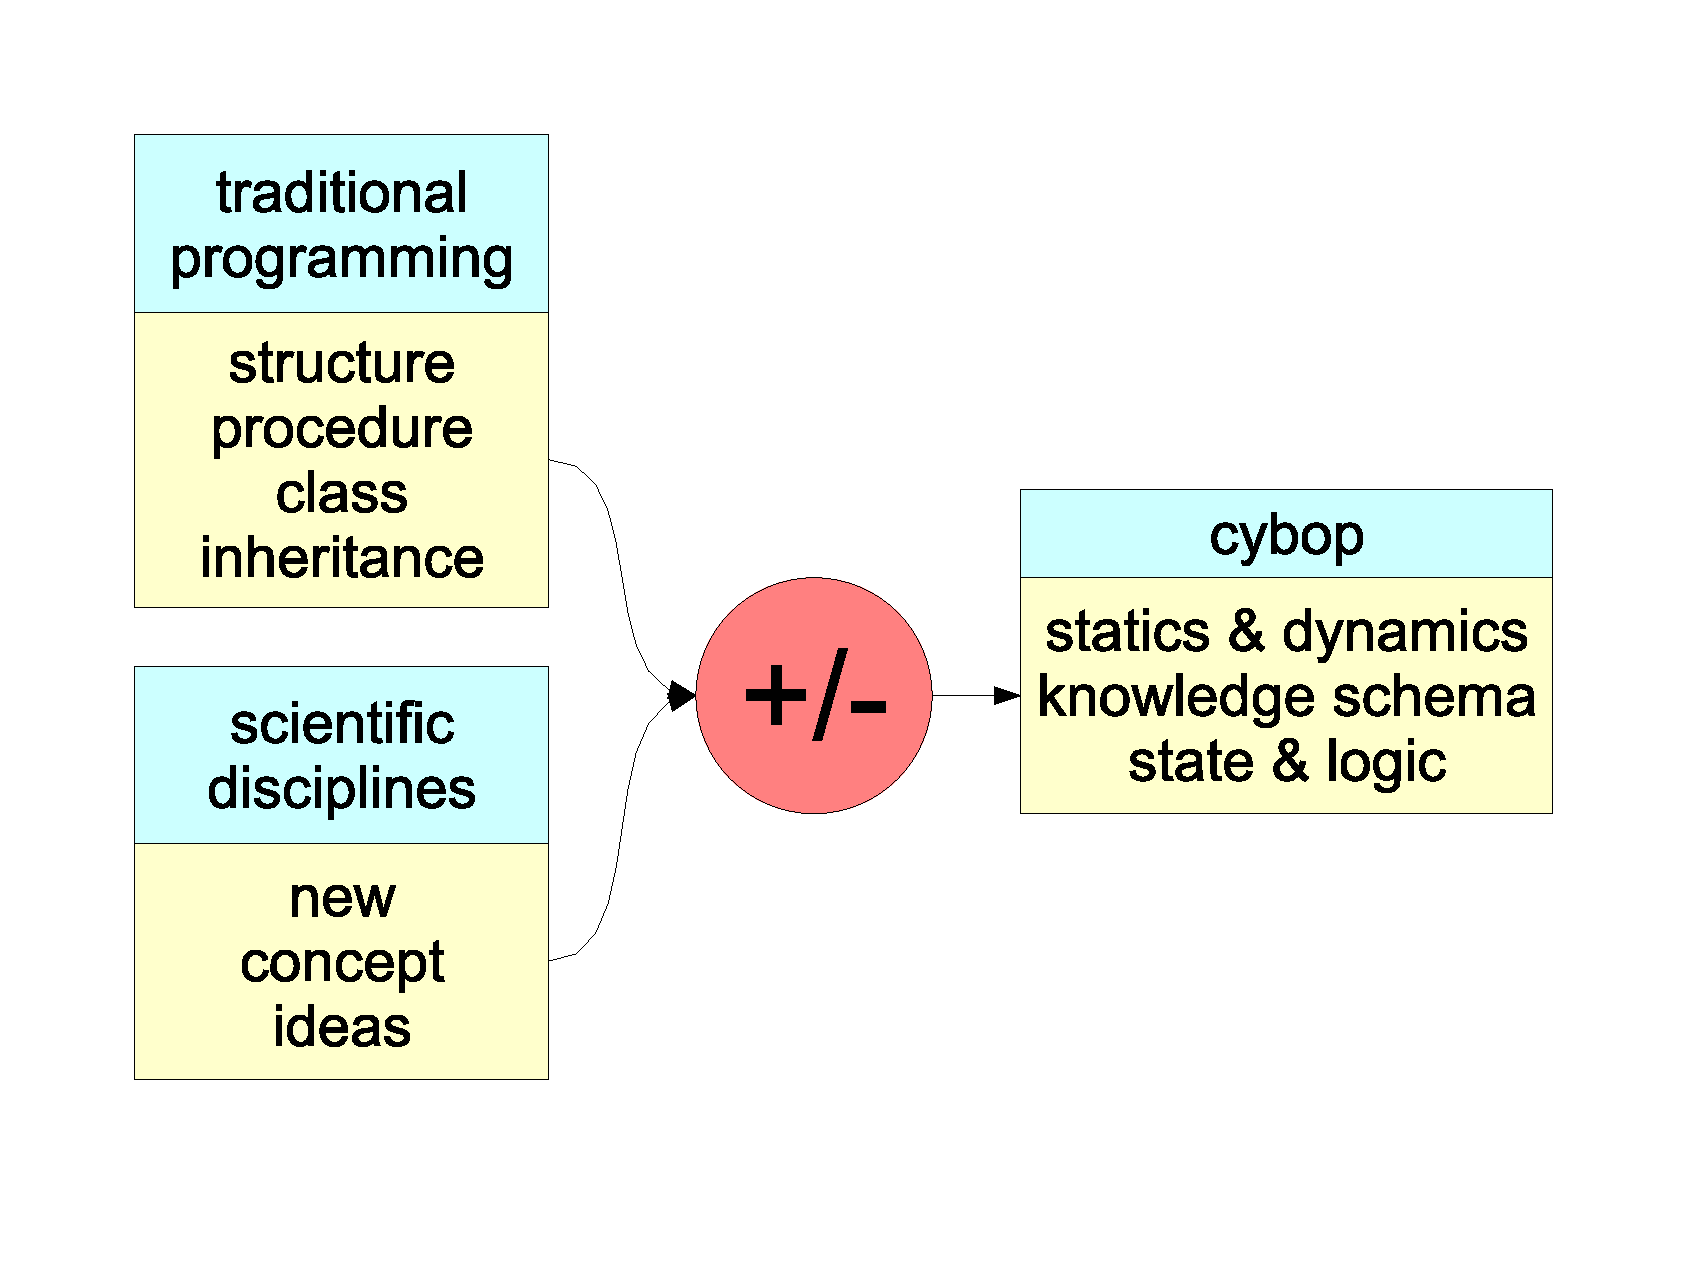
\includegraphics[scale=0.2]{vector/method.eps}
        \caption{Merger of Concepts}
        \label{method_figure}
    \end{center}
\end{figure}

However, these refactorings were only some of at least two dozens, since also
COP and the application of concerns, as well as other concepts applied later
(e.g. ontological structure implemented using the means of OOP) turned out to
have their deficiencies. According to the idea mentioned before, traditional
concepts were thus complemented, merged or revised with new concepts stemming
from other scientific disciplines (figure \ref{method_figure}), whenever a
classical design solution became unsatisfying.

Over the creation of a framework called \emph{ResMedLib}, which encapsulated
general application functionality, the prototype development finally ended up
in a complete reengineering: most of the functionality formerly residing in the
framework was moved into an interpreter (section \ref{cyboi_heading}) written
in the \emph{C} programming language; the actual application knowledge, on the
other hand, was put into special files, for which an
\emph{Extensible Markup Language} (XML)-based language (section
\ref{cybol_heading}) was defined.

Since problems did not occur in a predictable way, while developing the
mentioned prototype application, their presentation in order of appearance
would be rather confusing. An adapted structure of sections is therefore used
in this article, which first describes a number of observed discrepancies
(section \ref{existing_problems_heading}), then reflects on the most essential
new concepts (section \ref{reflexions_on_concepts_heading}), before it later
explains how these were implemented in practice (section
\ref{practical_proof_heading}).
